\subsection{Description}
%
Amazon Web Services is a subsidiary of Amazon that offers a metered pay-as-you-go cloud computing platforms and APIs to individuals, businesses, and governments. These web services for cloud computing include a range of simple abstract technical infrastructure and distributed computing building blocks and tools. 
%
\subsection{Services needed for CI/CD}
%
AWS offers more than 200 products and services, including computing, storage, database, networking, application services, deployment, management, analytics, machine learning, developer tools, and IoT tools. Among these, the most popular are Amazon Elastic Compute Cloud \textbf{(EC2)}, Amazon Simple Storage Service \textbf{(Amazon S3)}, Amazon Elastic Block Store \textbf{(EBS)}, Amazon Connect, and AWS Lambda.

\subsubsection{Amazon Elastic Computing Cloud (EC2)}
%
EC2 enables users to have a virtual cluster of computers accessible at any time via the Internet. It provides the most comprehensive computing platform, with  various options for processor, storage, networking, operating system, and purchase model. EC2 facilitates flexible application deployment by offering a web service that allows users to boot an Amazon Machine Image (AMI) and customize the virtual machine, which Amazon refers to as an "instance," with the software they prefer. The operating systems currently available to use with Amazon EC2 instances include: Amazon Linux, Windows Server 2012, CentOS 6.5 and Debian 7.4.
%

\subsubsection{AWS CodeCommit}
%
AWS CodeCommit is a fully managed source control service that hosts secure Git-based repositories. It makes it easy for teams to collaborate on code in a secure and highly scalable ecosystem. CodeCommit eliminates the need to operate our own source control system or worry about scaling its infrastructure. One can use CodeCommit to securely store anything from source code to binaries, and it works seamlessly with the existing Git tools.  
%

\subsubsection{Amazon Simple Storage Service (Amazon S3)}
%
Amazon Simple Storage Service is an object storage service that offers industry-leading scalability, data availability, security, and performance. 
%

\subsubsection{AWS CodeBuild}
%
AWS CodeBuild is a fully managed continuous integration service that compiles source code, runs tests, and produces software packages that are ready to deploy. CodeBuild provisions, manages, and scales our build servers continuously and processes multiple builds concurrently, so the builds are not left waiting in a queue.  
%

\subsubsection{AWS CodeDeploy}
%
AWS CodeDeploy is a fully managed deployment service that automates software deployments to a variety of computing services such as Amazon EC2, AWS Fargate, AWS Lambda, and on-premises servers. AWS CodeDeploy makes it easier to rapidly release new features, helps avoid downtime during application deployment, and handles the complexity of updating applications. 
%

\subsubsection{AWS CodePipeline}
%
AWS CodePipeline is a fully managed continuous delivery service that helps automate the release pipelines for fast and reliable application and infrastructure updates. CodePipeline automates the build, test, and deploy phases of the release process every time there is a code change, based on the release model we define. We can easily integrate AWS CodePipeline with third-party services such as GitHub or with our own custom plugin.
%

\subsubsection{AWS CloudFormation}
%
AWS CloudFormation gives us an easy way to model a collection of related AWS and third-party resources, provision them quickly and consistently, and manage them throughout their lifecycles, by treating infrastructure as code. A CloudFormation template describes our desired resources and their dependencies so we can launch and configure them together as a stack. We can use a template to create, update, and delete an entire stack as a single unit, as often as we need to, instead of managing resources individually. 
%

%
\subsection{CI-CD Process}
%
The following example uses two separate AWS accounts for development and production.
In summary, the example has the following workflow:

\begin{enumerate}
    \item A change or commit to the code in the CodeCommit application repository triggers CodePipeline with the help of a CloudWatch event.
    
    \item The pipeline downloads the code from the CodeCommit repository, initiates the Build and Test action using CodeBuild, and securely saves the built artifact on the S3 bucket.
    
    \item If the preceding step is successful, the pipeline triggers the Deploy in Dev action using CodeDeploy and deploys the app in dev account.
    
    \item If successful, the pipeline triggers the Deploy in Prod action using CodeDeploy and deploys the app in the prod account.
\end{enumerate}

The following diagram illustrates the workflow:

\begin{figure}[h]
    \centering
    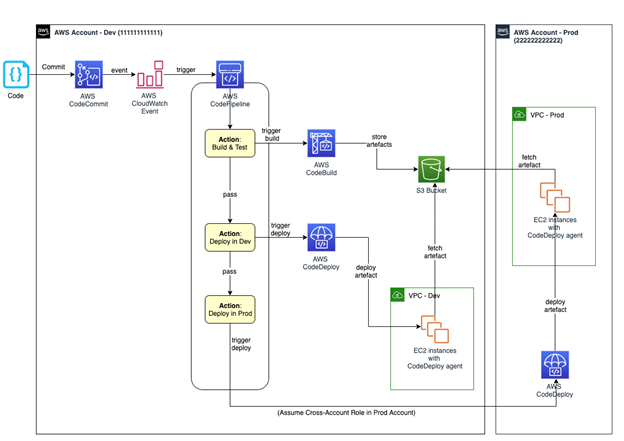
\includegraphics[width=\textwidth]{images/aws_cicd.png}
    \caption{Workflow of CI/CD pipeline in AWS.}
    \label{fig:aws_cicd}
\end{figure}



%
\subsection{Advantages}
%
\subsection{Disadvantages}
